\section{Simulation}
\begin{figure}[h]
    \centering
    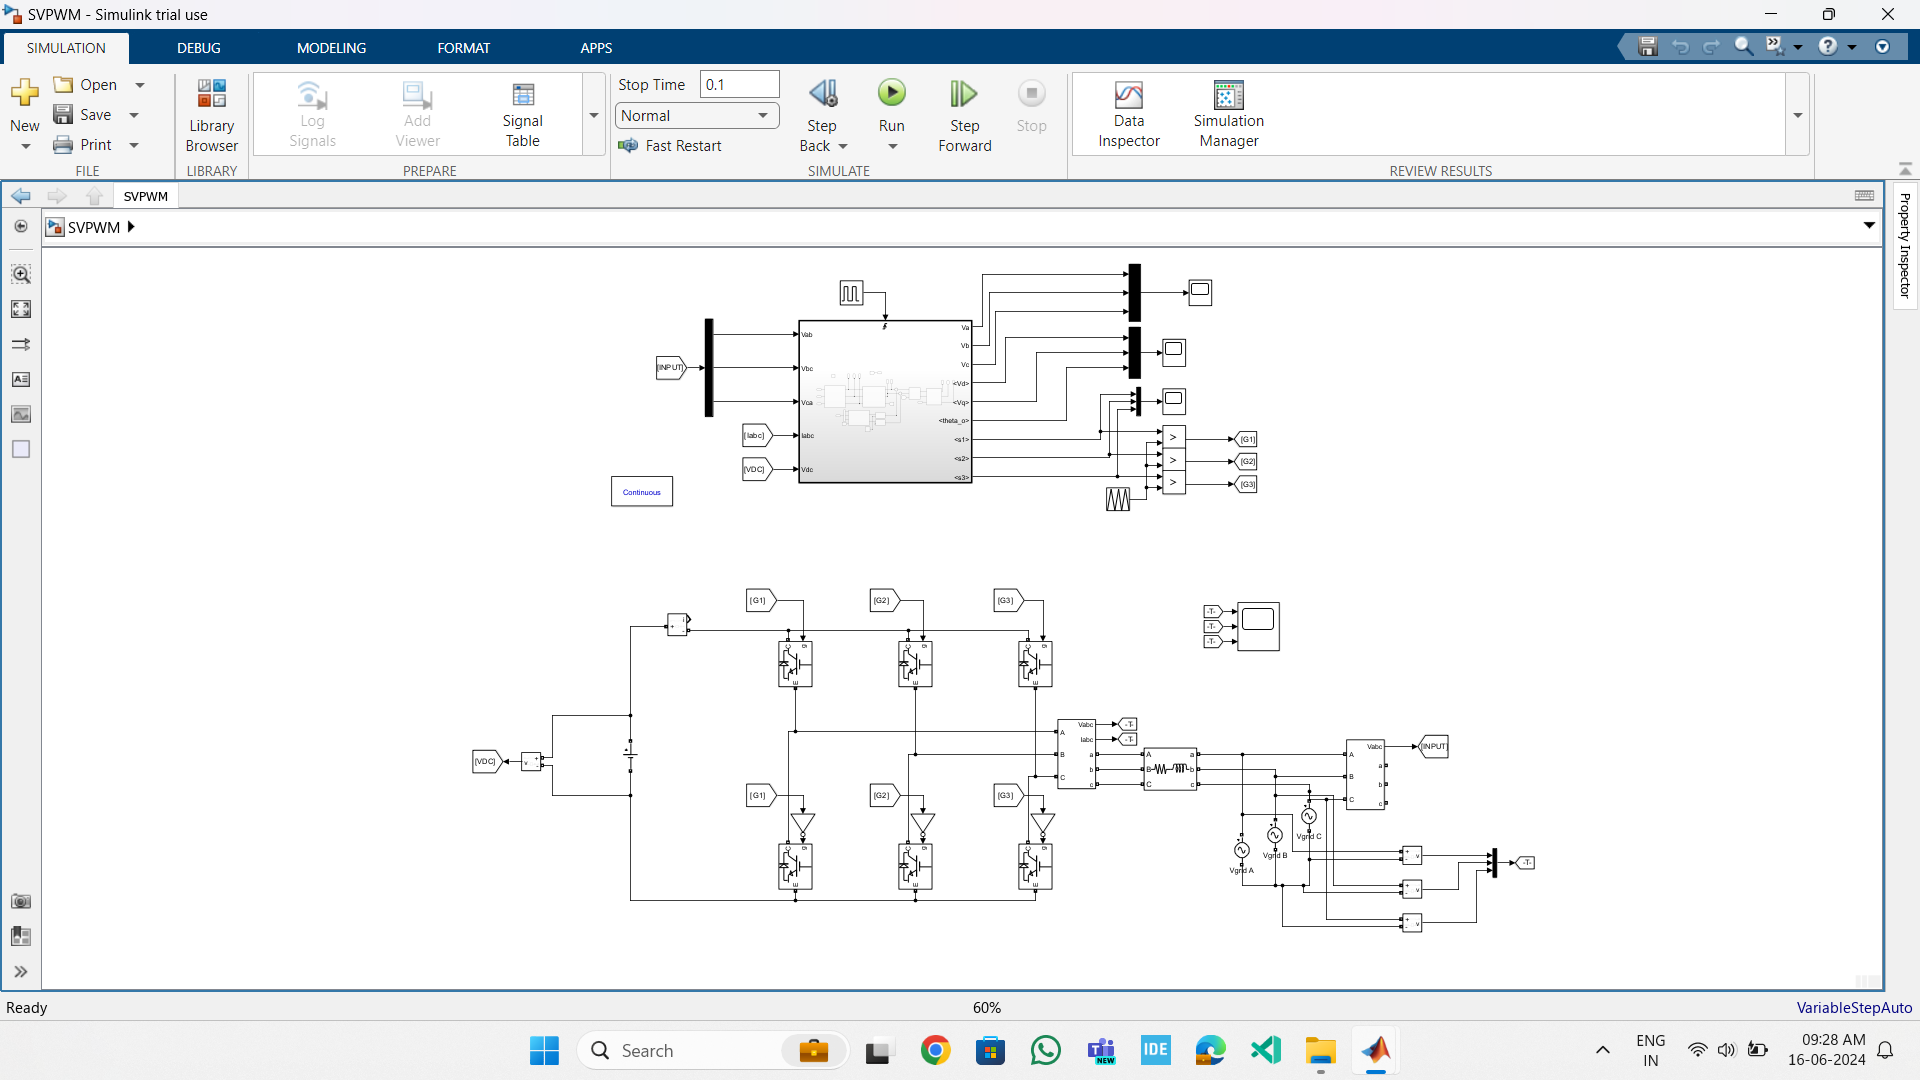
\includegraphics[width=\textwidth]{Whole Simulation.png}
    \caption{Simulation}
    \label{fig:Simulation}
\end{figure}
\noindent
Before initiating the design phase, it was imperative to conduct a
comprehensive simulation of the existing design using LtSpice. The simulation
setup involved creating the circuits for each individual sub-sections of the
circuit and understanding as well as analyzing the behavior of each and every
sub-circuit.

\subsection{MATLAB Function Blocks in Simulation}

\subsection{Control System}
\begin{figure}[h]
    \centering
    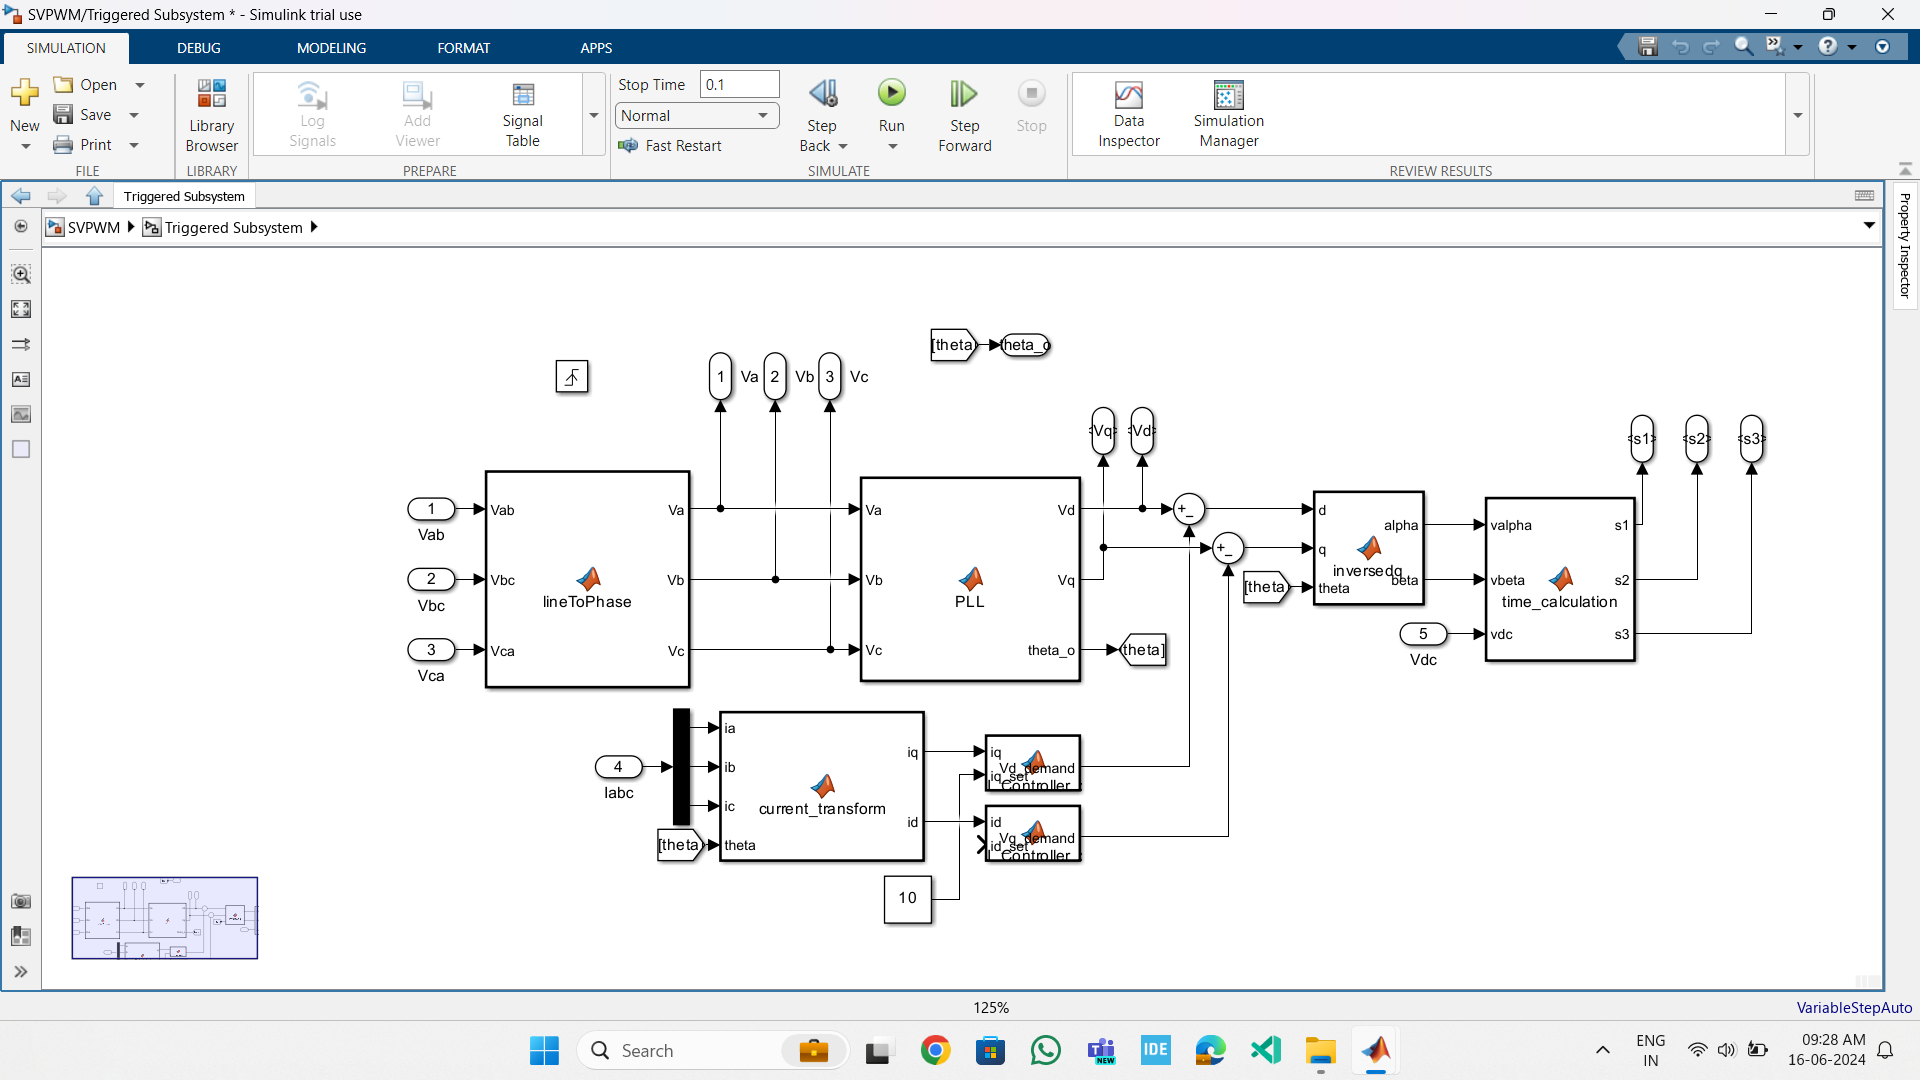
\includegraphics[width=\textwidth]{Control flow.png}
    \caption{Control System}
    \label{fig:Control System}
\end{figure}
\subsubsection{Voltage Transformation}


\subsubsection{Phase-Locked Loop (PLL)}


\subsubsection{Current Measurement and Transformation}


\subsubsection{Current Regulation}


\subsubsection{Voltage Calculation and Transformation}


\subsubsection{Gate Timing Calculation}


\subsection{Power System}
\begin{figure}[h]
    \centering
    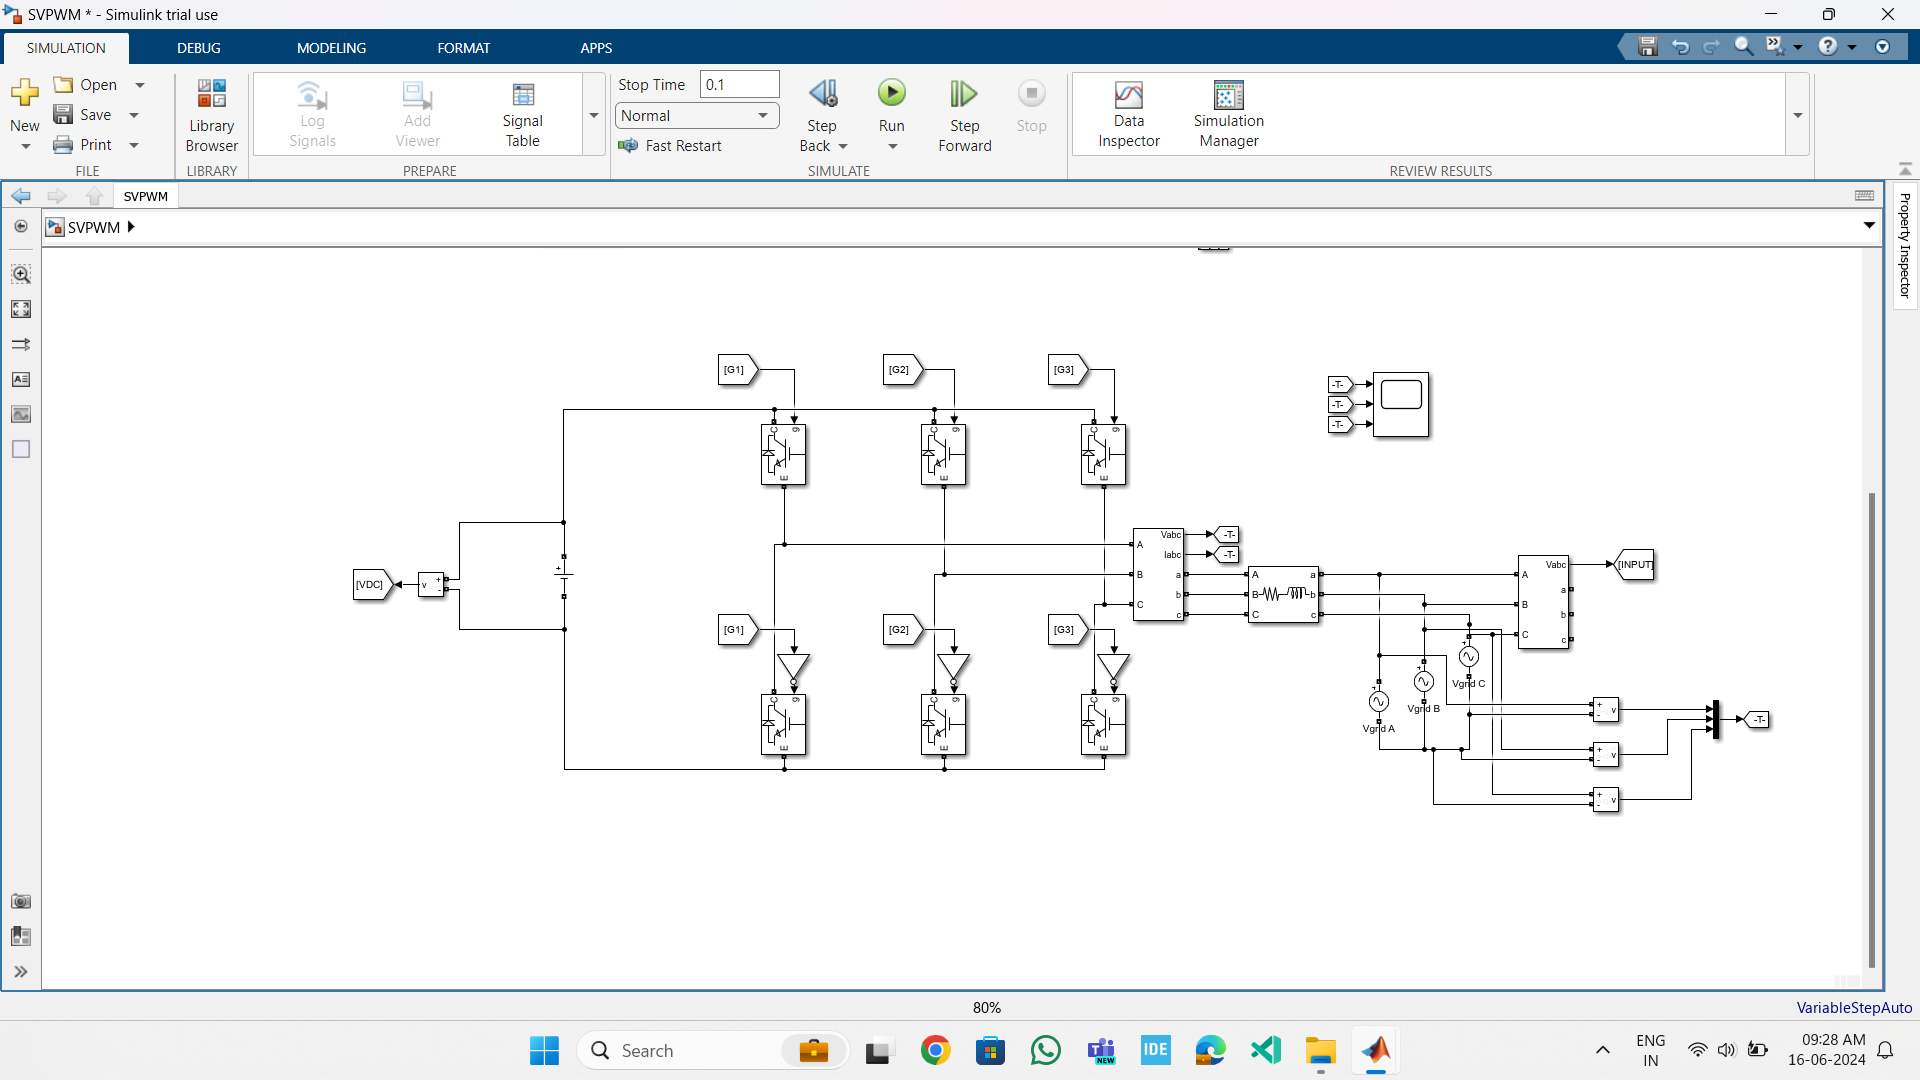
\includegraphics[width=\textwidth]{Power System.png}
    \caption{Power System}
    \label{fig:Power System}
\end{figure}

\subsubsection{Three-Phase AC Source}

\subsubsection{Three-Phase IGBT Bridge}


\section{Testing}


\subsection{Microcontroller Selection}

\subsection{Implementation of Voltage transform functions}

\subsection{Microcontroller Programming and Testing}

\begin{itemize}
    \item \textbf{ADC Sampling}: I utilized the ADC to sample the voltage values from the system. This real-time data acquisition was critical for the subsequent control processes.
    \item \textbf{Transformation and Modulation}: The sampled voltage values were processed using the previously developed Clarke and Park transform functions. This step generated the necessary parameters for Space Vector Modulation (SVM).
\end{itemize}
\noindent


\section{Calculation of LLC values}

\subsection{MATLAB Function Blocks in Simulation}

\subsection{Control System}

